\documentclass{article}
\usepackage{graphicx} % Required for inserting images

\title{CMM HW5}
\author{Xuanhao Lin}
\date{December 3 2023}

\begin{document}

\maketitle

\section{The Ising Model}
\subsection{Part 1}
\paragraph{
This part requires to plot magnetization M vs. Temperature T. For simplification, the Boltzmann constant $k_B$ is set to be 1. Given that \(J=1.5\), the analytical solution of the critical temperature of the Ising model should be \(T_c=3.402\). To equilibrate a system with a size of $n\times$$n$, \(10000n^2\) Monte Carlo sweeps are needed (very heavy computation).Figure 1 is the plot generated by Metropolis-Hastings algorithm. We can find that the $T_c$ of the system approximately equals to 3.402.
}
\begin{figure}[htbp]
    \centering
    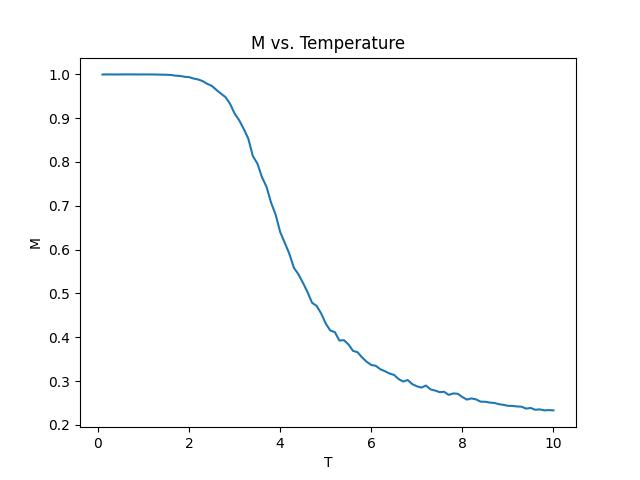
\includegraphics[width=0.5\linewidth]{Part1.jpeg}
    \caption{M vs. Temperature}
\end{figure}
\subsection{Part 2}
\paragraph{
Theoretically, the maximum heat capacity $C_{max}$ will appear at $T_c$. Due to the heavy computation of the large system (e.g. \(n=100\)), I only equilibrate the system at theoretical $T_c=3.402$ to find $C_{max}$. I haven't get the answer of the system with size of 200 and 500, since these sizes broke my PC system. The result is shown as Figure 2. However, the results look not convincing. Additionally, there are some result of C/N vs. T for systems with small sizes (Figure 3, Figure 4).
}
\begin{figure}[htbp]
    \centering
    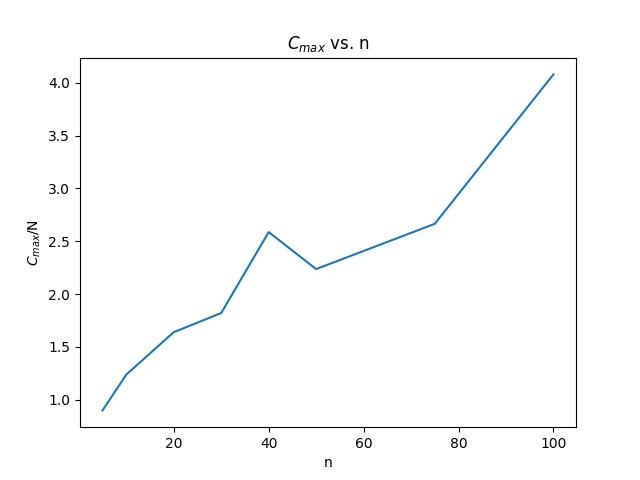
\includegraphics[width=0.5\linewidth]{Part2.jpeg}
    \caption{$C_{max}$/N vs. n}
\end{figure}
\begin{figure}[htbp]
    \centering
    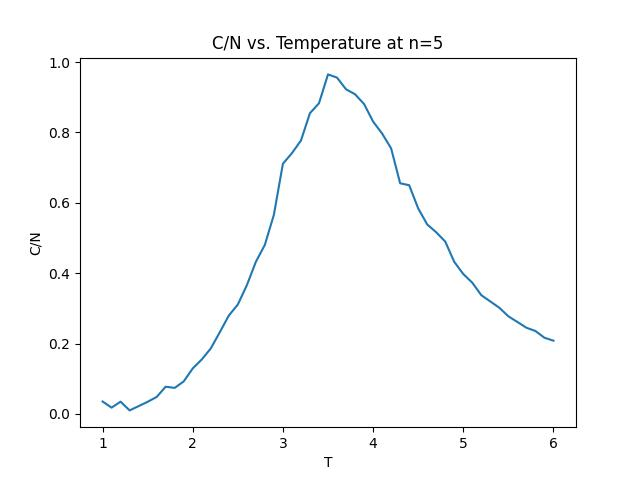
\includegraphics[width=0.5\linewidth]{Part2_n=5.jpeg}
    \caption{C/N vs. Temperature at n=5}
\end{figure}
\begin{figure}[htbp]
    \centering
    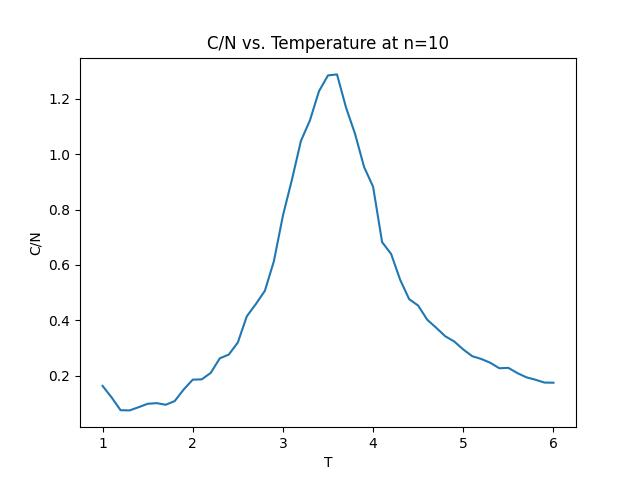
\includegraphics[width=0.5\linewidth]{Part2_n=10.jpeg}
    \caption{C/N vs. Temperature at n=10}
\end{figure}
\end{document}